\section{Introduction}

Diabetic Retinopathy (DR) is an eye disease that commonly
happens to diabetic patients. As the leading cause of blindness
in the working-age population of the developed world,
it is estimated to affect over millions of diabetic patients.
However, the vision impairment can be slowed or
even averted if diabetic retinopathy is detected in time.
The standard methodology for detecting DR is via manual
examination of the eye color fundus photographs by clinicians, which is yet still time-consuming and error-prone. Recently, with the development of machine learning (ML) techniques, researchers have proposed the use of ML to automatically detect DR using eye pictures of patients. This becomes an image classification task: takes a fundus photograph as input and classify it as either \texttt{DR} or \texttt{No DR}, using a ML model based on prior training knowledge~\cite{1}. A more sophisticated task will be to classify an image based
on the severity level of DR. Prior studies mostly focus on
developing ad-hoc algorithms or Convolutional Neural Network
(CNN) with customized architectures. These studies used various datasets and adopted different methodologies, for instance, tested both binary classification versus multi-class classification. Moreover, non-CNN based, traditional ML techniques such as decision tree and SVM \cite{C4.5,KNN,SVM}, rarely appeared in the
known studies.


\begin{figure}[t]
\centering
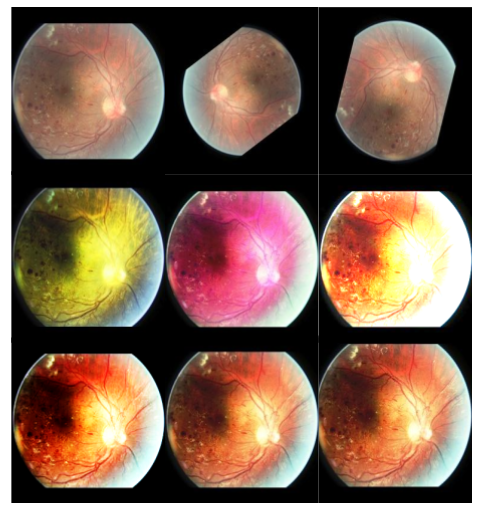
\includegraphics[width=0.4\textwidth]{thumbnail.png}
\caption{Different versions of sample image after augmentation}
\label{example}
\end{figure}

\begin{figure*}
\centering
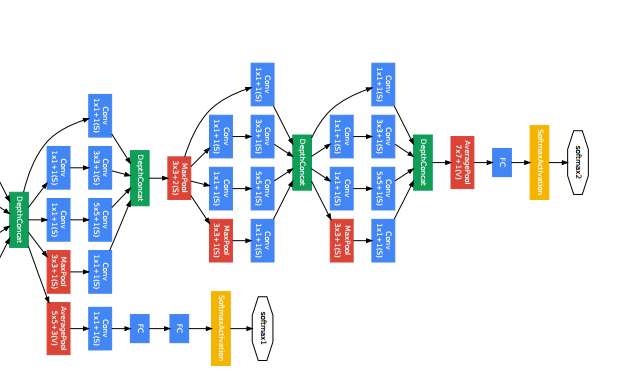
\includegraphics[width=0.8\textwidth]{googlenet_arch.png}
\caption{An overview of GoogLeNet architecture. We include only a portion of the architecture ; please refer to the paper for full architecture.}
\label{googlenet_arch}
\end{figure*}

In our experiments, we examine the performances of different ML models on detecting the severity level of DR (ranging from 0 - 4, where 0 stands for healthy and 4 stands for the most severe DR ). We start with image preprocessing to generate an augmented dataset using different augmentation methods. An example of different versions of selected image is shown in \figref{example}, with more details given in the later section. Then, we use conventional ML techniques to train on a combination of well-craft, generic features that have been demonstrated to be effective in previous studies, for example, the Histogram of Oriented Gradients~(HOG) and Local Binary Patterns~(LBP)~\cite{hog,lbp}. Finally, we explore the effectiveness of some CNN models such as GoogleNet and AlexNet~\cite{GoogleNet,AlexNet}. 

\textbf{Summary of observations.} We find that: 
\begin{itemize}
\item The weighted average accuracy of traditional ML methods with generic features are only slightly better than random-guess. The accuracy of the best-performing classifier is only about 29\%.
\item Without the need of feature selection and parameter tuning, GoogleNet and AlexNet can easily achieve an accuracy above 90\%. The results suggest some advanced CNN networks are very powerful at feature extraction and image classification. 
\end{itemize}

Our paper is organized in the following manner: In the background 
section we introduce the related work on DR detection using 
traditional ML methods and using CNN separately. Then, we describe the dataset we use and how we perform data augmentation. Finally, we explain the experimental 
design, and provide an evaluation of results for traditional ML methods and CNNs respectively. 


